\documentclass[]{../template/Report}%方括号内写yuxi即生成预习报告\documentclass[yuxi]{../template/Report}
\settemplatedir{../template/}%设置模板路径

\exname{金属材料杨氏模量的测定} %实验名称
\extable{} %实验桌号
\instructor{} %指导教师
\class{} %班级
\name{} %姓名
\stuid{} %学号

\nyear{} %年
\nmonth{} %月
\nday{} %日
\nweekday{} %星期几,e.g. \nweekday{三}
\daypart{}%上午/下午

\redate{} %如有实验补做,补做日期
\resitu{} %情况说明:

\begin{document}
\maketitle%输出封面

\section{预习报告}
\subsection{实验综述}
杨氏模量用于量化材料在弹性形变范围内的刚度。根据胡克定律,在弹性限度内,金属材料的应力
(单位面积所受的力,$F/S$)和应变(外力作用下的相对形变,$\Delta L /L$)成正比,定义该比例系数为杨氏模量
\[E = \frac{F \cdot L}{S \cdot \Delta L}\]

为测量杨氏模量,采用光杠杆法。实验仪器如\cref{shiyanzhuangzhi}所示。

\begin{figure}[htbp]
    \centering
    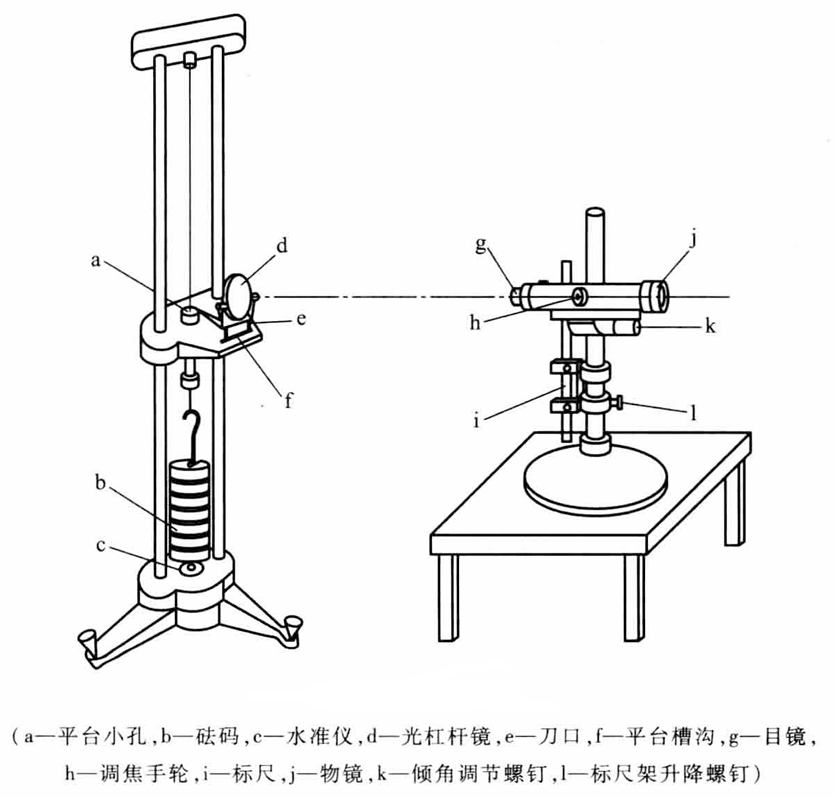
\includegraphics[width=0.75\textwidth]{shiyanzhuangzhi.png}
    \caption{金属材料杨氏模量测定的实验装置}
    \label{shiyanzhuangzhi}
\end{figure}

光杠杆镜是一块带有三足的平面镜,如\cref{guanggangganjing}所示。
它的三个足尖$O_1,O_2,O_3$构成等腰三角形,顶点$O_3$到底边的距离为$b$标尺通过平面镜反射后,在望远镜中成像。
则可在望远镜中观察到标尺的像。望远镜中十字叉丝线处在标尺上的刻度初始值记为$s_0$。

\begin{figure}[htbp]
    \centering
    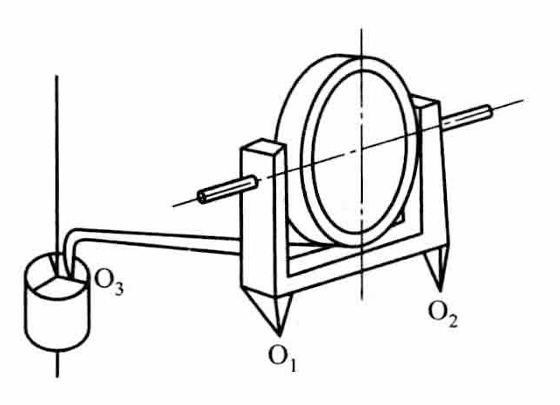
\includegraphics[width=0.4\textwidth]{guanggangganjing.png}
    \caption{光杠杆镜}
    \label{guanggangganjing}
\end{figure}

保持$O_1,O_2$在一个平台上,$O_3$下降$\Delta L$,则平面镜转过$\theta$角,望远镜中十字叉丝线处在标尺上的刻度值变为$s_1$。光路图如\cref{guanglutu}所示。
记望远镜中读到十字叉丝线处在标尺的刻度值变化为$\Delta s = s_1 - s_0$,由几何关系$\frac{\Delta s}{D} = \tan 2 \theta \approx 2 \theta$,$\frac{\Delta L}{b} = \tan \theta \approx \theta$。
由此可得
\[\Delta s = \frac{2D}{b} \Delta L\]
其中$D$为标尺与光杠杆镜镜面间的距离。由于$\frac{2D}{b} \gg 1$,所以望远镜中标尺读数$\Delta s$比钢丝实际伸长量$\Delta L$放大了$\frac{2D}{b}$倍,$\frac{2D}{b}$称为光杠杆常数。

\begin{figure}[htbp]
    \centering
    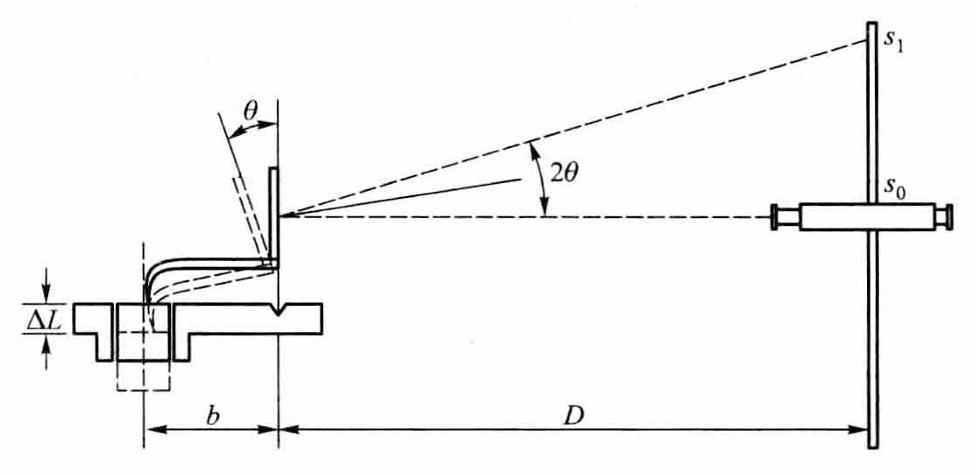
\includegraphics[width=0.6\textwidth]{guanglutu.png}
    \caption{本实验的光路图}
    \label{guanglutu}
\end{figure}

又因为钢丝截面积$S = \frac{1}{4} \pi d^2$($d$为钢丝直径),代入杨氏模量计算式中就得到
\[\bar{E} = \frac{8DmgL}{\pi d^2 b \cdot \Delta s}\]

不确定度计算原理见“误差分析”部分。


本实验的步骤如下:
\begin{enumerate}
    \item 预备实验,用螺旋测微计(在不同部位)测量金属丝直径$d$,用米尺测量金属丝原长$L$,用卷尺测量标尺到镜面的距离$D$,用游标卡尺测量光杠杆镜前后脚垂直距离$b$(将三只脚在白纸上压出凹痕,用尺画出两前脚连线,再用游标卡尺读出后脚到连线垂直距离)。都多次测量取平均值。
    \item 调节好实验仪器,使支架铅直,金属丝拉直,夹具无接触;反射镜面竖直,望远镜对焦、共轴、无视差;
    \item 连续逐个增加砝码,然后减少砝码,记录砝码质量和标尺读数(8组不同重量的数据);对于测得的相应标尺读数$s_i$和$s_i'$取平均,然后用逐差法求得$\Delta s_i = \frac{s_{i+4} - s_i}{4} , i=0,1,2,3$;
    \item 按照上述理论推导计算杨氏模量和不确定度。
\end{enumerate}
\subsection{实验重点}

\begin{enumerate}
    \item 理解杨氏模量的定义及测量原理;
    \item 掌握用光杠杆法测量微小长度的原理;
    \item 学习用逐差法处理实验数据,并分析不确定度。
\end{enumerate}

\subsection{实验难点}

\begin{enumerate}
    \item 初次接触,可能面临仪器使用不熟练的情况,如无法从望远镜观察到尺子的像;
    \item 精密实验,容易产生粗大误差,如金属丝夹头未夹紧、仪器支柱不铅直、触碰使光杠杆镜足尖移动等;
    \item 数据处理的技巧不够熟练,可能产生错误。
\end{enumerate}

\begin{fullreportonly}
% \section{原始数据}
% \begin{figure}[h]
%     \centering
%     \includegraphics[width=0.8\textwidth]{data.jpg}
%     \caption{实验数据}
%     \label{data}
% \end{figure}


\section{结果与分析}
\subsection{数据处理与结果}
预备实验$D,b,L,d$的测量值,及计算得到的平均值如\cref{yubeidata}所示。
\begin{table}[H]
    \centering
    \caption{测得$D,b,L,d$的相关量}
    \begin{tabular}{C{.25\textwidth}C{.13\textwidth}C{.13\textwidth}C{.13\textwidth}C{.13\textwidth}}
    \toprule
      & $D/\si{mm}$  & $b/\si{mm}$ & $L/\si{mm}$ & $d/\si{mm}$ \\
    \midrule
    1 & 1356.1 & 71.80 & 1048.9 & 0.667 \\
    2 & 1355.5 & 71.00 & 1048.0 & 0.678 \\
    3 & 1356.0 & 70.50 & 1049.2 & 0.681 \\
    4 & 1353.9 & 71.38 & 1049.1 & 0.685 \\
    5 & 1354.9 & 71.60 & 1045.0 & 0.684 \\
    平均值$\bar{x}$ & 1355.3 & 71.26 & 1048.0 & 0.679 \\
    \bottomrule
    \end{tabular}
    \label{yubeidata}
\end{table}

正式实验中,测得标尺读数和对应砝码质量如\cref{zhengshidata}所示。

\begin{table}[H]
    \centering
    \caption{实验标尺读数和砝码质量}
    \begin{tabular}{C{.15\textwidth}C{.07\textwidth}C{.07\textwidth}C{.07\textwidth}C{.07\textwidth}C{.07\textwidth}C{.07\textwidth}C{.07\textwidth}C{.07\textwidth}}
    \toprule
    次数 & 1 & 2 & 3 & 4 & 5 & 6 & 7 & 8 \\
    \midrule
    $m/\si{kg}$ & 2.00 & 3.00 & 4.00 & 5.00 & 6.00 & 7.00 & 8.00 & 9.00 \\
    增砝码时$s/\si{mm}$ & 80.0 & 75.0 & 70.1 & 65.2 & 62.9 & 58.2 & 53.5 & 47.9 \\
    减砝码时$s'/\si{mm}$ & 89.0 & 81.9 & 76.7 & 70.9 & 66.8 & 61.0 & 52.9 & 48.0 \\
    平均值$\bar{s}\si{mm}$ & 84.5 & 78.5 & 73.4 & 68.1 & 64.9 & 59.6 & 53.2 & 48.0 \\
    \bottomrule
    \label{zhengshidata}
    \end{tabular}
\end{table}

使用逐差法计算,$\Delta s_1 = \SI{19.6}{mm}$,$\Delta s_2 = \SI{18.9}{mm}$,$\Delta s_3 = \SI{20.2}{mm}$,$\Delta s_4 = \SI{20.1}{mm}$。
平均值$\overline{\Delta s} = \SI{19.7}{mm}$。$\Delta s$对应的质量变化$\Delta m = \SI{4.00}{kg}$。

查表得,杭州市的重力加速度为$\SI{9.7936}{m \per s^2}$,计算得到,钢丝的杨氏模量为
\[\bar{E} = \frac{8DmgL}{\pi d^2 b \cdot \Delta s} = \SI{2.19 E 11}{Pa}\]

\subsection{误差分析}

对每个测量量,其A类不确定度$\Delta_A(x) = \sqrt{\frac{1}{n\left(n-1\right)} \sum\limits_{k=1}^n \left(x_k - \bar{x}\right)^2}$,B类不确定度$\Delta_b (x) = \frac{\Delta_\text{仪}}{p}$(本实验中取$p=\sqrt{3}$),合成不确定度$\Delta (x) = \sqrt{\Delta_A(x)^2 + \Delta_B(x)^2}$

本实验相对不确定度公式可由不确定度传递公式导出,即
\[E_r = \frac{\Delta E}{\bar{E}} = \sqrt{\left(\frac{\Delta m}{\overline{m}}\right)^2 +\left(\frac{\Delta L}{\overline{L}}\right)^2 + \left(\frac{\Delta D}{\overline{D}}\right)^2 + \left(\frac{2\Delta d}{\overline{d}}\right)^2 + \left(\frac{\Delta b}{\overline{b}}\right)^2 + \left(\frac{\Delta \left(\Delta s\right)}{\overline{\Delta s}}\right)^2}\]
最终结果为$E = \bar{E} \pm \Delta E$,单位为$\si{\Pa}$。

根据以上原理,计算各测量量实验误差如\cref{result}所示。
\begin{table}[H]
    \centering
    \caption{各测量量实验误差及结果}
    \begin{tabular}{C{.2\textwidth}C{.13\textwidth}C{.13\textwidth}C{.13\textwidth}C{.13\textwidth}C{.13\textwidth}}
    \toprule
      & $D/\si{mm}$  & $b/\si{mm}$ & $L/\si{mm}$ & $d/\si{mm}$ & $\Delta s /\si{mm}$\\
    \midrule
    平均值$\bar{x}$ & 1355.3 & 71.26 & 1048.0 & 0.679 & 19.7 \\
    A类不确定度$\Delta_A(x)$ & 0.4 & 0.23 & 0.8 & 0.003 & 0.3\\
    仪器允差$\Delta_\text{仪}$& 0.5 & 0.02 & 0.5 & 0.004 & 0.2\\
    总不确定度$\Delta x$ & 0.5 & 0.23 & 0.8 & 0.004  & 0.3\\
    测量值$x$ & $1355.3\pm0.5$ & $71.26\pm0.23$ & $1048.0\pm0.8$ & $0.679\pm0.004$ & $19.7\pm0.3$\\
    \bottomrule
    \end{tabular}
    \label{result}
\end{table}

砝码的质量不确定度$\Delta m = \frac{\Delta_\text{仪} m}{\sqrt{3}} = \SI{0.289}{g}$。

于是计算得杨氏模量测定的相对不确定度
\[E_r = \frac{\Delta E}{\bar{E}} = \sqrt{\left(\frac{\Delta m}{\overline{m}}\right)^2 +\left(\frac{\Delta L}{\overline{L}}\right)^2 + \left(\frac{\Delta D}{\overline{D}}\right)^2 + \left(\frac{2\Delta d}{\overline{d}}\right)^2 + \left(\frac{\Delta b}{\overline{b}}\right)^2 + \left(\frac{\Delta \left(\Delta s\right)}{\overline{\Delta s}}\right)^2}
=0.020\]

从而$\Delta E = E_r \bar{E} = \SI{0.04E11}{Pa}$,最终测量结果为$2.19 \pm 0.04 \times 10^{11} \si{Pa}$。

本实验的误差来源主要有
\begin{enumerate}
    \item 测量$L$和$D$时产生的误差,在视差外,还存在因肉眼无法保证尺子完全水平或垂直产生的误差;
    \item 测量$d$时产生的误差,实验中发现金属丝粗细不均匀,并且不同部位粗细差别较大;
    \item 测量$b$时产生的误差,主要是作图产生的误差;
    \item 测量$s$时产生的误差,金属丝一直在振动,导致读数不准确;
    \item 砝码质量标称值与实际值间存在一定偏差。
\end{enumerate}

\subsection{实验探讨}
本实验介绍了利用光杠杆法测定金属丝杨氏模量的方法,我掌握了杨氏模量的定义和测量方法,并提高了数据处理能力。
实验中最困难的就是调整光路使标尺出现在望远镜中,经过助教耐心的讲解和帮助,我成功克服了这一困难。

\section{思考题}

\subsection{伸长法测量钢丝的杨氏弹性模量中需要测量哪些物理量?分别用什么仪器测量?应估读到哪一位?}
\begin{table}[H]
	\centering
	\begin{tabular}{C{.2\textwidth}C{.2\textwidth}C{.2\textwidth}}
		\toprule
		物理量 & 测量仪器 & 应估读到的位数 \\
		\midrule
		金属丝总长$L$ & 米尺 & 0.1mm \\
		光杠杆长臂$D$ & 卷尺 & 0.1mm \\
		光杠杆短臂$b$ & 游标卡尺 & 不估读 \\
		金属丝直径$d$ & 螺旋测微仪 & 0.001mm \\
		标尺刻度值变化$\Delta S$ & 标尺 & 0.1mm \\
		\bottomrule
	\end{tabular}
\end{table}


\subsection{加减砝码测量钢丝伸长量的过程中,如何及时检查所测得的数据?}

根据测量原理,$s$和$m$应近似成线性关系,增减砝码时,$s$应线性变化。
每次测量时,可以估测$s$的变化趋势,若明显是非线性变化,则说明实验装置和操作可能有错。
例如金属丝夹头松动,光杠杆移位或砝码多放/少放等。

\subsection{从光杠杆的放大倍数考虑,增大$D$与减小$b$都可以增加放大倍数,那么它们有何不同?是否可以增大D从而无限制地增大放大倍数,光杠杆放大倍数增大有无限制?}
增大$D$是通过移动望远镜或光杠杆镜所在支架实现的,较易操作实现;而减小$b$是通过更换光杠杆镜实现的,光杠杆镜型号有限,且不一定适配平台上的小孔和槽沟,实现较为困难。

不可以增大$D$从而无限制地增大放大倍数。其原因,也即光杠杆放大倍数受限制的原因包括:
\begin{enumerate}
    \item 实验室空间存在限制,不能无限移动望远镜或支架;
    \item $D$很大时,在望远镜中观察平面镜反射标尺的像将极为困难;
    \item $D$很大时,$D$的测量难度和精度也加大,容易增加误差;
    \item $D$很大时,放大倍数很大,容易导致$s$在标尺上的读数超量程,无法读数;
    \item $D$很大时,光线衰减将比较严重,很难在望远镜中发现标尺明亮易读的像。
\end{enumerate}

\end{fullreportonly}
\insertnotes
\end{document}